

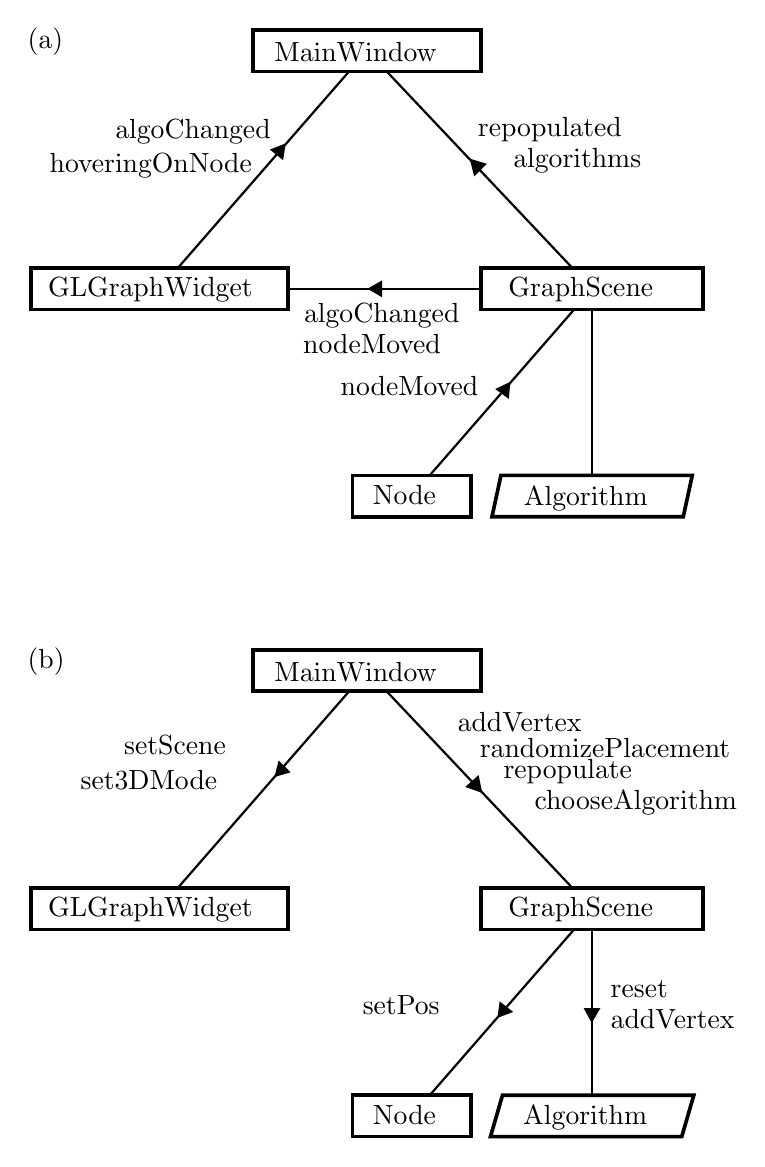
\begin{tikzpicture}[y=0.80pt, x=0.8pt,yscale=-1, inner sep=0pt, outer sep=0pt]
\begin{scope}[shift={(-112.55702,-213.37695)}]
  \begin{scope}[cm={{0.60244614,0.0,0.0,0.60244614,(61.856524,54.195329)}}]
    \path[draw=black,line width=1.328pt,rounded corners=0.0000cm]
      (268.2596,281.6544) rectangle (438.9601,312.6544);
    \path[fill=black] (284.14697,305.60364) node[above right] (text3003) {MainWindow
      };
  \end{scope}
  \begin{scope}[cm={{0.60244614,0.0,0.0,0.60244614,(41.49929,104.70602)}}]
    \path[fill=black] (148.19138,401.63339) node[above right] (text2991)
      {GLGraphWidget       };
    \path[draw=black,line width=1.328pt,rounded corners=0.0000cm]
      (135.3776,376.3655) rectangle (328.3015,407.3655);
  \end{scope}
  \begin{scope}[cm={{0.60244614,0.0,0.0,0.60244614,(88.967165,105.34863)}}]
    \path[fill=black] (414.52719,400.70734) node[above right] (text2995) {GraphScene
      };
    \path[draw=black,line width=1.328pt,rounded corners=0.0000cm]
      (393.9723,375.2989) rectangle (560.6322,406.2989);
  \end{scope}
  \begin{scope}[cm={{0.60244614,0.0,-0.13122252,0.60244614,(154.0838,136.35127)}}]
    \path[fill=black] (428.1041,505.48331) node[above right] (text2987) {Algorithm
      };
    \path[draw=black,line width=1.328pt,rounded corners=0.0000cm]
      (405.2505,479.1763) rectangle (548.6769,510.1763);
  \end{scope}
  \path[draw=black,line join=miter,line cap=butt,line width=0.800pt]
    (189.3056,331.4460) -- (266.7520,242.5528);
  \path[draw=black,line join=miter,line cap=butt,line width=0.800pt]
    (283.7097,242.5528) -- (367.6938,331.4460);
  \path[draw=black,line join=miter,line cap=butt,line width=0.800pt]
    (326.3143,340.7839) -- (239.2832,340.7839);
  \path[draw=black,line join=miter,line cap=butt,line width=0.800pt]
    (376.5161,350.1218) -- (376.5161,425.0292);
  \path[fill=black] (246.43787,358.36713) node[above right] (text3059)
    {algoChanged     };
  \path[fill=black] (246.03421,370.05441) node[above right] (text3063) {nodeMoved
    };
  \path[cm={{0.60244614,0.0,0.0,0.60244614,(219.19954,185.07318)}},draw=black,fill=black,line
    join=miter,line cap=butt,miter limit=4.00,line width=1.328pt]
    (102.3179,254.4263) -- (102.2747,262.3632) -- (95.4227,258.3573) -- cycle;
  \path[cm={{0.59608163,0.08733863,-0.08733863,0.59608163,(198.29375,115.77633)}},draw=black,fill=black,line
    join=miter,line cap=butt,miter limit=4.00,line width=1.328pt]
    (102.3179,254.4263) -- (102.2747,262.3632) -- (95.4227,258.3573) -- cycle;
  \path[cm={{-0.69799145,0.17382972,-0.18444507,-0.71573379,(441.95326,452.94883)}},draw=black,fill=black,line
    join=miter,line cap=butt,miter limit=4.00,line width=1.097pt]
    (102.3179,254.4263) -- (102.2747,262.3632) -- (95.4227,258.3573) -- cycle;
  \path[fill=black] (161.1712,275.12494) node[above right] (text3118) {algoChanged
    };
  \path[fill=black] (131.48926,290.81223) node[above right] (text3122)
    {hoveringOnNode     };
  \begin{scope}[cm={{0.60244614,0.0,0.0,0.60244614,(80.129239,88.883392)}}]
    \path[fill=black] (327.60049,579.53265) node[above right] (text3128) {Node
      };
    \path[draw=black,line width=1.328pt,rounded corners=0.0000cm]
      (312.2591,557.9682) rectangle (401.1372,588.9682);
  \end{scope}
  \path[draw=black,line join=miter,line cap=butt,line width=0.800pt]
    (303.1524,425.0292) -- (368.3843,350.1218);
  \path[cm={{0.58190708,0.05230551,-0.04887953,0.5983474,(291.49485,226.59278)}},draw=black,fill=black,line
    join=miter,line cap=butt,miter limit=4.00,line width=1.351pt]
    (102.3179,254.4263) -- (102.2747,262.3632) -- (95.4227,258.3573) -- cycle;
  \path[fill=black] (262.92914,388.73416) node[above right] (text3146) {nodeMoved
    };
  \path[fill=black] (324.94656,274.44034) node[above right] (text3150)
    {repopulated     };
  \path[fill=black] (121.5652,235.30273) node[above right] (text3889) {(a)     };
  \begin{scope}[cm={{0.60244614,0.0,0.0,0.60244614,(61.856524,334.19533)}}]
    \path[draw=black,line width=1.328pt,rounded corners=0.0000cm]
      (268.2596,281.6544) rectangle (438.9601,312.6544);
    \path[fill=black] (284.14697,305.60364) node[above right] (text3901) {MainWindow
      };
  \end{scope}
  \begin{scope}[cm={{0.60244614,0.0,0.0,0.60244614,(41.49929,384.70602)}}]
    \path[fill=black] (148.19138,401.63339) node[above right] (text3907)
      {GLGraphWidget       };
    \path[draw=black,line width=1.328pt,rounded corners=0.0000cm]
      (135.3776,376.3655) rectangle (328.3015,407.3655);
  \end{scope}
  \begin{scope}[cm={{0.60244614,0.0,0.0,0.60244614,(88.967165,385.34863)}}]
    \path[fill=black] (414.52719,400.70734) node[above right] (text3915) {GraphScene
      };
    \path[draw=black,line width=1.328pt,rounded corners=0.0000cm]
      (393.9723,375.2989) rectangle (560.6322,406.2989);
  \end{scope}
  \begin{scope}[cm={{0.60244614,0.0,-0.17496336,0.60244614,(175.72135,416.35127)}}]
    \path[fill=black] (428.44839,505.48331) node[above right] (text3923) {Algorithm
      };
    \path[draw=black,line width=1.328pt,rounded corners=0.0000cm]
      (405.2505,479.1763) rectangle (548.6769,510.1763);
  \end{scope}
  \path[draw=black,line join=miter,line cap=butt,line width=0.800pt]
    (189.3056,611.4460) -- (266.7520,522.5528);
  \path[draw=black,line join=miter,line cap=butt,line width=0.800pt]
    (283.7097,522.5528) -- (367.6938,611.4460);
  \path[draw=black,line join=miter,line cap=butt,line width=0.800pt]
    (376.5161,630.1218) -- (376.5161,705.0292);
  \path[cm={{-0.58532849,-0.14258998,0.14258998,-0.58532849,(257.79281,723.57069)}},draw=black,fill=black,line
    join=miter,line cap=butt,miter limit=4.00,line width=1.328pt]
    (102.3179,254.4263) -- (102.2747,262.3632) -- (95.4227,258.3573) -- cycle;
  \path[cm={{0.70569892,-0.13927625,0.14900577,0.72394207,(214.68757,391.73552)}},draw=black,fill=black,line
    join=miter,line cap=butt,miter limit=4.00,line width=1.097pt]
    (102.3179,254.4263) -- (102.2747,262.3632) -- (95.4227,258.3573) -- cycle;
  \path[fill=black] (165.1712,551.12494) node[above right] (text3951) {setScene
    };
  \path[fill=black] (145.48926,566.81226) node[above right] (text3955) {set3DMode
    };
  \begin{scope}[cm={{0.60244614,0.0,0.0,0.60244614,(80.129239,368.88339)}}]
    \path[fill=black] (327.60049,579.53265) node[above right] (text3961) {Node
      };
    \path[draw=black,line width=1.328pt,rounded corners=0.0000cm]
      (312.2591,557.9682) rectangle (401.1372,588.9682);
  \end{scope}
  \path[draw=black,line join=miter,line cap=butt,line width=0.800pt]
    (303.1524,705.0292) -- (368.3843,630.1218);
  \path[cm={{0.35985131,-0.46028117,0.47594756,0.3658999,(177.46665,618.17186)}},draw=black,fill=black,line
    join=miter,line cap=butt,miter limit=4.00,line width=1.351pt]
    (102.3179,254.4263) -- (102.2747,262.3632) -- (95.4227,258.3573) -- cycle;
  \path[fill=black] (272.92914,668.73413) node[above right] (text3971) {setPos
    };
  \path[fill=black] (315.80371,540.58319) node[above right] (text3975) {addVertex
    };
  \path[fill=black] (121.5652,515.30273) node[above right] (text3979) {(b)     };
  \path[fill=black] (325.80371,552.58319) node[above right] (text3983)
    {randomizePlacement     };
  \path[fill=black] (336.51801,564.58319) node[above right] (text3987) {repopulate
    };
  \path[fill=black] (340.94656,288.44034) node[above right] (text3991) {algorithms
    };
  \path[fill=black] (350.51801,578.58319) node[above right] (text3995)
    {chooseAlgorithm     };
  \path[cm={{0.50323671,0.29682408,-0.30078027,0.51955755,(403.81881,503.95313)}},draw=black,fill=black,line
    join=miter,line cap=butt,miter limit=4.00,line width=1.351pt]
    (102.3179,254.4263) -- (102.2747,262.3632) -- (95.4227,258.3573) -- cycle;
  \path[fill=black] (384.92914,660.73413) node[above right] (text4001) {reset
    };
  \path[fill=black] (384.92914,674.73413) node[above right] (text4005) {addVertex
    };
\end{scope}

\end{tikzpicture}
